\chapter{Searching for a good model}

Atrium segmentations from CT data (experimental setup + results).

\section{Triplanar method, compressed patches}

\section{Generating the datasets}

How did I generate the training and testing datasets?

\section{Hyper-parameter search}

\subsection{General approach to looking for a good model}

Describe the base model. Describe how I am undertaking the hyper-parameter search. Describe the dice coefficient.

\subsection{varying datasets type}

Describe the atrium box approach. Conjecture that the improved results were because of a higher concentration of training examples in the boundary regions.

\begin{figure}
\centering
\begin{minipage}{0.45\textwidth}
\centering
\fbox{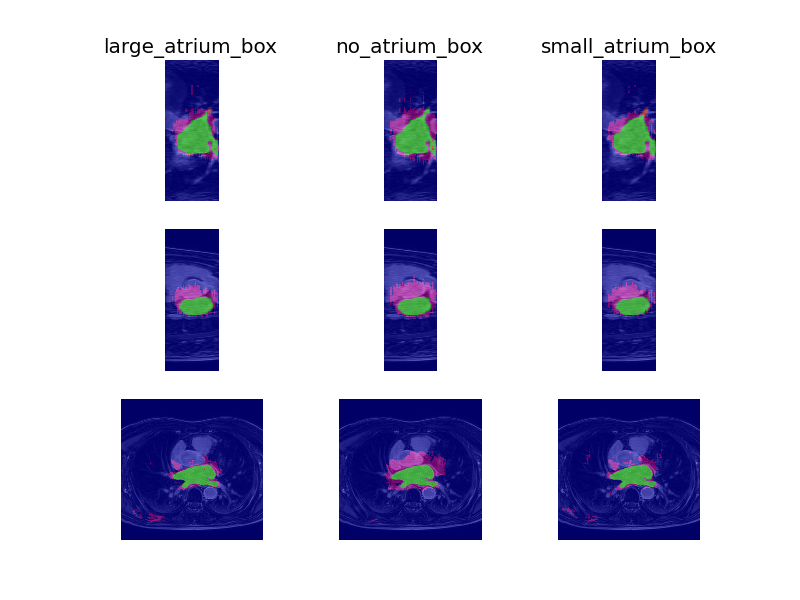
\includegraphics[height=60mm, width=70mm]{Chapter3/mask_results_varying_dataset.png}}
\end{minipage}\hfill
\hspace{-1cm}
\begin{minipage}{0.45\textwidth}
\centering
\fbox{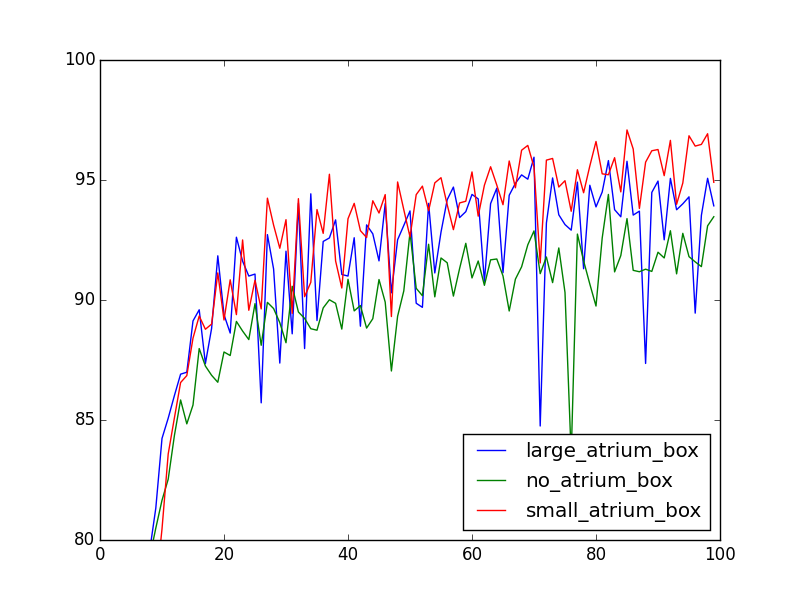
\includegraphics[height=60mm, width=70mm]{Chapter3/test_dice_coefficient_plots_varying_dataset.png}}
\end{minipage}
\caption{Left: grey scale slices from a CT scan taken in the transversal, saggital and coronal planes. Right: illustration of the triplanar}
\end{figure}

\subsection{varying number of convolutional layers}

We tried 3 different architectures with 1, 2, 3 convolutional layers while keeping all the other parameters the same. We find that having more than 1 doesn't improve the results much. Of note that I have no max pooling in the second convolutional layer to not decrease the number of features too much.

\subsection{varying number of connected layers}

Having settled on an architecture with 1 convolutional layer, we trained 3 CNNs with 1, 2, and 3 connected layers. Having more than 1 connected layer doesn't make a difference.

\subsection{varying number of feature maps}

So now the focus is on finding the right number of feature maps for the convolutional layer. We tried 16/32/64/128 and it seems having 64 feature maps gives the best bang for the buck.

\subsection{varying the number of hidden units}

We now vary the number of hidden units in the connected layer, trying 100, 200, 500, 1000 and 1500. 200 is best...

\subsection{varying the activation function}

We experimented with different types of activation function: ReLU, Tanh, Sigmoid. Doing it with ReLU is better...

\subsection{varying the type of pooling}

We also tried different types of pooling: Max pooling and average pooling. No difference, so we stuck with Max pooling

\subsection{varying the learning rate}

Tried different learning rates: 0.01, 0.05, 0.1, 0.5, 1. It seems that 0.1 is best. Having a learning rate of 1 doesn't train the network.  We omitted the results.

\subsection{varying the momentum}

Tried different momentums: 0, 0.01, 0.05, 0.1. Having momentum actually slightly improves the test results!

\subsection{varying the data size}

Tried a number of dataset sizes: 400000, 1000000, 3000000: No improved result from the increased data size.


